\input{../preamble.tex}

\SetDate[11/03/2026]

\begin{document}
\pagestyle{fancy}
\fancyhead[L]{Première spécifique}
\fancyhead[C]{\textbf{Dérivation}}
\fancyhead[R]{\today}





\exe{,difficulty=1}{
	Considérons la fonction $f$ donnée graphiquement ci-dessous.
	\begin{enumerate}
		\item Quel est le signe de $f(2)$ ?
		\item Quel est le signe de $f'(2)$ ?
		\item Tracer tangente à $\C_f$ en $x=2$ et en déduire approximativement la valeur de $f'(2)$.
		\item Tracer tangente à $\C_f$ en $x=1$ et en déduire approximativement la valeur de $f'(1)$.
	\end{enumerate}

	\begin{center}
	\begin{tikzpicture}[>=stealth, scale=1]
	\begin{axis}[xmin=-.1, xmax=3, ymin=-4, ymax=4, axis x line=middle, axis y line=middle, axis line style=-, grid=both, xtick distance = 1, minor tick num = 1, clip=true]
		\addplot[BLUE_E, very thick, domain=0:3, samples=50] {1*(x-1)^3 - 2}  node[pos = .5, above=15pt] {$\C_{f}$};
	\end{axis}
	\end{tikzpicture}
	\end{center}

}{exe:tangente-graphique}{
}


\exe{,difficulty=1}{
	On considère un objet de position $f(t)$ et de vitesse $f'(t)$ aux temps $t \in \D = [0;3]$.
	La courbe représentative de $f'$ est donnée ci-dessous.

	\begin{enumerate}
		\item Compléter le tableau de signes de $f'$ de variations de $f$.
		\item Peut-on déduire le maximum et le minimum de $f$ sur $\D$ uniquement à l'aide de ses variations ?
	\end{enumerate}

	\begin{center}
	\begin{tikzpicture}[>=stealth, scale=1]
	\begin{axis}[xmin=-.1, xmax=3, ymin=-4, ymax=4, axis x line=middle, axis y line=middle, axis line style=-, grid=both, xtick distance = 1, minor tick num = 1]
		
		% (f')
		%\addplot[myr, very thick, domain =-2:3, samples=50] {(x+1)*x*(x-2)+.5}  node[pos = .77, right=2pt] {$\C_{f'}$};
		\addplot[RED_E, very thick, domain=0:3, samples=50] {3*(x-1.5)^2 - 3}  node[pos = .23, above=15pt] {$\C_{f'}$};
	\end{axis}
	\end{tikzpicture}
	\hfill
	\begin{tikzpicture}
		\tkzTabInit
		 %[lgt=3,espcl=1.5]
	       		{$x$ / 1 , Signe de $f'(x)$ / 1, Variation de $f(x)$ / 2}
	       		{,,}
	\end{tikzpicture}
	\end{center}
}{exe:lecture-graphique}{
}

\exe{}{
	Donner la fonction dérivée de chaque fonction suivante.
	\begin{multicols}{2}
	\begin{enumerate}
		\item $f(x) = 3x$
		\item $g(x) = -x^2$
		\item $h(x) = 2x^3+4$
		\item $F(x) = 1-x+x^2$
		\item $G(x) = x^3 + 3x - 6$
		\item $H(x) = 2x^2 - x^3$
	\end{enumerate}
	\end{multicols}
}{exe:derivation}{
}

\newpage


\exe{,difficulty=1}{
	On considère la fonction $f$ du troisième degré définie sur le domaine $\D=\left[0;5\right]$ :
		\[ f(x) = x^3 - 6x^2 + 9x-5. \]
	%On connait $f'$, la dérivée de $f$, donnée par
	%	\[ f'(x) = 3x^2 - 12x + 9. \]
	
	\begin{enumerate}
		\item Donner $f'(x)$.
		\item Montrer que $f'(x) = 3(x-1)(x-3)$.
		\item Remplir le tableau de signes et de variations de la figure \ref{fig:var-signe}.
		\item Compléter les variations avec les images de $f$ aux bornes de $\D$ ainsi qu'aux extrema locaux.
		\item En déduire le maximum et le minimum de $f$ sur $\D$.
		\item Utiliser le tableau pour esquisser $\C_f$ dans le repère figure \ref{fig:Cf}.
	\end{enumerate}
}{exe:variations-d3}{
}


\begin{figure}[h]
	\centering	
	\begin{tikzpicture}
		\tkzTabInit
		 %[lgt=3,espcl=1.5]
	       		{$x$ / 1 , Signe de $x-1$ / 1, Signe de $x-3$ / 1, Signe de $f'(x)$ / 1, Variation de $f(x)$ / 2}
	       		{0,,,,5}
	\end{tikzpicture}
	\caption{Tableau de variations de $f$ et de signes de $f'$.}
	\label{fig:var-signe}
\end{figure}

\begin{figure}[h]
	\centering
	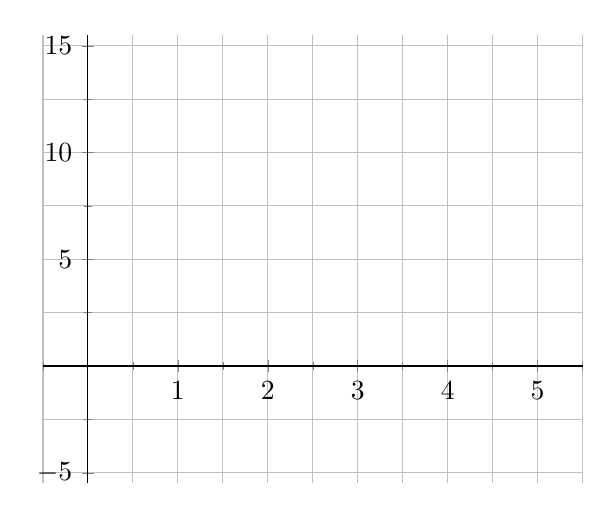
\begin{tikzpicture}[scale=1]
	\begin{axis}[
		xmin = -.5, xmax=5.5,
		ymin=-5.5, ymax=15.5,
		axis x line=middle, 
		axis y line=middle, 
		axis line style=-,
		grid = both, % xlabel={$x$}, ylabel={$f(x)$},
		minor tick num = 1,
	%xtick = {0, 0.2, ..., 1.4},
	%ytick = {-1, -0.5, 0, .5, 1.5},
	]
	%\addplot[domain=.5:5, myb] {x^3 - 6*x^2 + 9*x-5};
	\end{axis}
	\end{tikzpicture}
	\caption{Graphe approximatif de $\C_f$.}
	\label{fig:Cf}
\end{figure}



\exe{,difficulty=1}{
	On considère la fonction $f$ du troisième degré définie sur $\R$ :
		\[ f(x) = 3 - 6x - 3x^2 - x^3. \]
	%On connait $f'$, la dérivée de $f$, donnée par
	%	\[ f'(x) = -3x^2 - 6x - 6. \]

	\begin{enumerate}
		\item Montrer que $f'(x) = -3 - 3(x+1)^2$.
		\item En déduire que $f$ est décroissante sur $\R$.
		\item Donner le minimum et le maximum de $f$ sur $[-3 ; 10]$.
	\end{enumerate}

}{exe:variation-carre}{
}




%%%%%%%%%%%%

\newpage
\fancyhead[C]{\textbf{Solutions}}
\shipoutAnswer

\end{document}
